\documentclass[tikz,border=3pt]{standalone}
\usepackage{mathptmx}
\usepackage{amsmath}
\usetikzlibrary{arrows.meta,calc}
\definecolor{pvblue}{HTML}{0072B2}
\definecolor{pvorange}{HTML}{D55E00}
\definecolor{pvink}{HTML}{374151}
\definecolor{pvmuted}{HTML}{AEB8C2}
\begin{document}
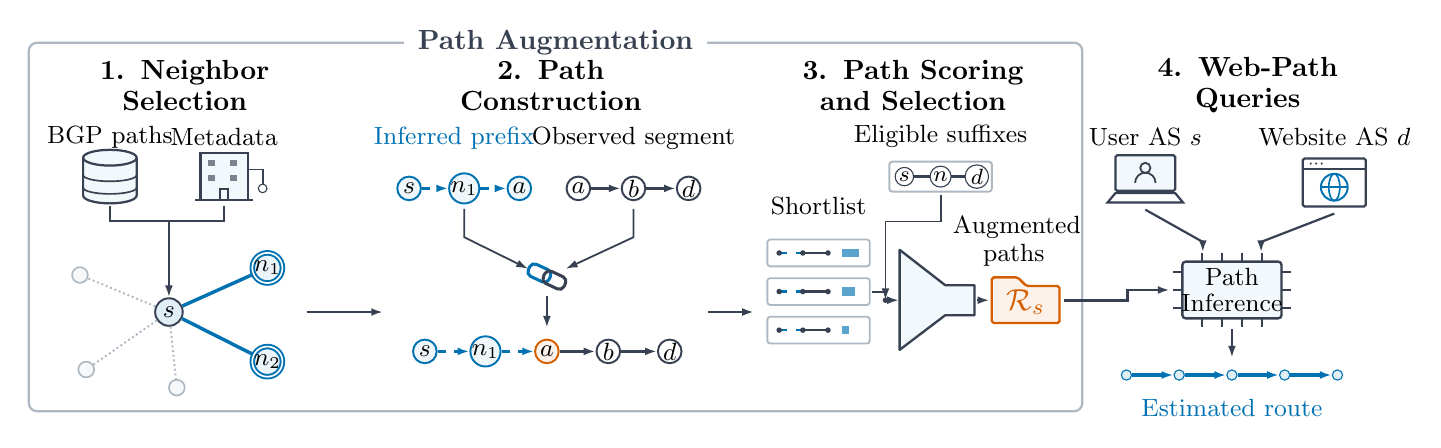
\begin{tikzpicture}[
 font=\fontsize{9.2}{10.6}\selectfont,
 >={Latex[length=1.5mm,width=1.0mm]},
 flow/.style={->,draw=pvink,line width=.8pt},
 inferred/.style={->,draw=pvblue,line width=1pt,dashed},
 observed/.style={->,draw=pvink,line width=1pt},
 heading/.style={font=\fontsize{9.6}{11.3}\selectfont\bfseries,
   align=center,text width=3.7cm,inner sep=0pt},
 small/.style={font=\fontsize{8.8}{10.1}\selectfont,align=center,inner sep=1pt},
 as/.style={circle,draw=pvink,fill=white,line width=.7pt,
   minimum size=.35cm,inner sep=0pt,font=\fontsize{8.7}{9.5}\selectfont},
 chosen/.style={as,draw=pvblue,fill=pvblue!8,double,double distance=.6pt},
 faint/.style={circle,draw=pvmuted,fill=pvmuted!10,
   minimum size=.20cm,inner sep=0pt,line width=.6pt},
 route/.style={as,minimum size=.30cm},
 pics/database/.style={code={
   \path[draw=pvink,fill=pvblue!5,line width=.8pt]
    (-.34,.24)--(-.34,-.24)
    arc[start angle=180,end angle=360,x radius=.34,y radius=.10]
    --(.34,.24) arc[start angle=0,end angle=180,x radius=.34,y radius=.10];
   \draw[pvink,line width=.8pt] (-.34,.24)
    arc[start angle=180,end angle=360,x radius=.34,y radius=.10];
   \draw[pvink,line width=.6pt] (-.34,.02)
    arc[start angle=180,end angle=360,x radius=.34,y radius=.08];
   \draw[pvink,line width=.6pt] (-.34,-.14)
    arc[start angle=180,end angle=360,x radius=.34,y radius=.08];
 }},
 pics/metadata/.style={code={
   \draw[pvink,fill=pvblue!5,line width=.8pt] (-.30,-.30) rectangle (.30,.30);
   \draw[pvink,line width=.7pt] (-.37,-.30)--(.37,-.30);
   \foreach \x in {-.16,.12} {\foreach \y in {-.02,.17} {
    \path[fill=pvink!65] (\x-.045,\y-.04) rectangle (\x+.045,\y+.04);}}
   \draw[pvink,line width=.7pt] (-.055,-.30)--(-.055,-.16)--(.055,-.16)--(.055,-.30);
   \draw[pvink,line width=.65pt] (.30,.09)--(.49,.09)--(.49,-.15);
   \node[circle,draw=pvink,fill=white,minimum size=.11cm,inner sep=0pt] at (.49,-.15) {};
 }},
 pics/laptop/.style={code={
   \draw[pvink,fill=pvblue!5,line width=.8pt,rounded corners=.6pt]
    (-.38,-.08) rectangle (.38,.37);
   \path[draw=pvink,fill=white,line width=.8pt]
    (-.48,-.23)--(.48,-.23)--(.38,-.11)--(-.38,-.11)--cycle;
   \draw[pvink,line width=.65pt] (0,.21) circle[radius=.065];
   \draw[pvink,line width=.65pt] (-.13,.02) arc[start angle=180,end angle=0,radius=.13];
 }},
 pics/website/.style={code={
   \draw[pvink,fill=white,line width=.8pt,rounded corners=.6pt]
    (-.40,-.28) rectangle (.40,.33);
   \draw[pvink,line width=.65pt] (-.40,.20)--(.40,.20);
   \foreach \x in {-.30,-.23,-.16} {\fill[pvink] (\x,.265) circle[radius=.015];}
   \draw[pvblue,line width=.7pt] (0,-.035) circle[radius=.17];
   \draw[pvblue,line width=.6pt] (0,-.035) ellipse[x radius=.07,y radius=.17];
   \draw[pvblue,line width=.6pt] (-.17,-.035)--(.17,-.035);
 }},
 pics/library/.style={code={
   \path[draw=pvorange,fill=pvorange!8,line width=.85pt,rounded corners=.7pt]
    (-.43,-.29)--(-.43,.29)--(-.10,.29)--(.01,.18)--(.43,.18)--(.43,-.29)--cycle;
   \node[font=\fontsize{11}{12}\selectfont,text=pvorange] at (0,-.025) {$\mathcal R_s$};
 }},
 pics/chip/.style={code={
   \foreach \x in {-.38,-.13,.13,.38} {
    \draw[pvink,line width=.7pt] (\x,.36)--(\x,.47);
    \draw[pvink,line width=.7pt] (\x,-.36)--(\x,-.47);}
   \foreach \y in {-.23,0,.23} {
    \draw[pvink,line width=.7pt] (-.63,\y)--(-.75,\y);
    \draw[pvink,line width=.7pt] (.63,\y)--(.75,\y);}
   \draw[pvink,fill=pvblue!5,line width=.85pt,rounded corners=1.2pt]
    (-.63,-.36) rectangle (.63,.36);
   \node[align=center,font=\fontsize{8.8}{9.5}\selectfont] {Path\\Inference};
 }},
 pics/link/.style={code={
   \draw[pvblue,line width=1.1pt,rotate=-25,rounded corners=1.8pt]
    (-.25,-.085) rectangle (.04,.085);
   \draw[pvink,line width=1.1pt,rotate=-25,rounded corners=1.8pt]
    (-.04,-.085) rectangle (.25,.085);
 }}
]
% Steps 1--3 jointly augment paths; Web-path queries remain outside.
\draw[draw=pvmuted,line width=.8pt,rounded corners=3pt]
  (-.48,-.58) rectangle (12.90,4.10);
\node[fill=white,text=pvink,inner xsep=5pt,inner ysep=1pt,
  font=\fontsize{10.4}{11.8}\selectfont\bfseries]
  at (6.21,4.10) {Path Augmentation};
\node[heading] at (1.50,3.56) {1. Neighbor\\Selection};
\node[heading] at (6.15,3.56) {2. Path\\Construction};
\node[heading] at (10.75,3.56) {3. Path Scoring\\and Selection};
\node[heading] at (15.00,3.56) {4. Web-Path\\Queries};

% Public routing archive and interconnection metadata.
\node[small] at (.55,2.90) {BGP paths};
\node[small] at (2.00,2.90) {Metadata};
\pic at (.55,2.40) {database};
\pic at (2.00,2.40) {metadata};
\draw[pvink,line width=.7pt] (.55,2.03)--(.55,1.84)--(1.30,1.84);
\draw[pvink,line width=.7pt] (2.00,2.03)--(2.00,1.84)--(1.30,1.84);

% Bold links and double rings encode selected exits in grayscale as well.
\node[as,fill=pvblue!12] (src) at (1.30,.68) {$s$};
\node[chosen] (n1) at (2.55,1.24) {$n_1$};
\node[chosen] (n2) at (2.55,.05) {$n_2$};
\node[faint] (f1) at (.17,1.15) {};
\node[faint] (f2) at (.25,-.05) {};
\node[faint] (f3) at (1.40,-.28) {};
\draw[flow] (1.30,1.84)--(src.north);
\draw[pvblue,line width=1.25pt] (src)--(n1);
\draw[pvblue,line width=1.25pt] (src)--(n2);
\foreach \n in {f1,f2,f3} {\draw[pvmuted,densely dotted,line width=.7pt] (src)--(\n);}
\draw[flow,line width=1pt] (3.05,.68)--(4.02,.68);

% The same anchor occurs in a predicted prefix and a measured segment.
\node[small,text=pvblue] at (4.92,2.89) {Inferred prefix};
\node[small] at (7.20,2.89) {Observed segment};
\node[route,draw=pvblue,fill=pvblue!6] (ps) at (4.35,2.25) {$s$};
\node[route,draw=pvblue,fill=pvblue!6] (pn) at (5.05,2.25) {$n_1$};
\node[route,draw=pvblue,fill=pvblue!6] (pa) at (5.75,2.25) {$a$};
\draw[inferred] (ps)--(pn); \draw[inferred] (pn)--(pa);
\node[route] (oa) at (6.50,2.25) {$a$};
\node[route] (ob) at (7.20,2.25) {$b$};
\node[route] (od) at (7.90,2.25) {$d$};
\draw[observed] (oa)--(ob); \draw[observed] (ob)--(od);
\draw[flow,line width=.65pt] (5.05,1.99)--(5.05,1.63)--(5.86,1.23);
\draw[flow,line width=.65pt] (7.20,1.99)--(7.20,1.63)--(6.34,1.23);
\pic at (6.10,1.13) {link};
\draw[flow] (6.10,.88)--(6.10,.48);
\node[route,draw=pvblue,fill=pvblue!6] (js) at (4.55,.18) {$s$};
\node[route,draw=pvblue,fill=pvblue!6] (jn) at (5.32,.18) {$n_1$};
\node[route,draw=pvorange,fill=pvorange!8] (ja) at (6.10,.18) {$a$};
\node[route] (jb) at (6.88,.18) {$b$};
\node[route] (jd) at (7.66,.18) {$d$};
\draw[inferred] (js)--(jn); \draw[inferred] (jn)--(ja);
\draw[observed] (ja)--(jb); \draw[observed] (jb)--(jd);
\draw[flow,line width=1pt] (8.15,.68)--(8.73,.68);

% Route cards and score bars represent the synthetic shortlist.
\node[small] at (9.55,2.03) {Shortlist};
\foreach \y/\bar in {1.43/.22,.94/.16,.45/.09} {
 \begin{scope}[shift={(9.55,\y)}]
  \draw[pvmuted,fill=white,rounded corners=1pt,line width=.65pt]
    (-.65,-.17) rectangle (.65,.17);
  \draw[pvblue,line width=.8pt,dashed] (-.50,0)--(-.20,0);
  \draw[pvink,line width=.8pt] (-.20,0)--(.12,0);
  \foreach \x in {-.50,-.20,.12} {\fill[pvink] (\x,0) circle[radius=.035];}
  \path[fill=pvblue!65] (.30,-.055) rectangle ({.30+\bar},.055);
 \end{scope}
}

% Eligible full suffixes merge BEFORE the selector, never after admission.
\node[small] at (11.10,2.91) {Eligible suffixes};
\begin{scope}[shift={(11.10,2.40)}]
 \draw[pvmuted,fill=white,rounded corners=1pt,line width=.7pt]
   (-.65,-.19) rectangle (.65,.19);
 \draw[pvink,line width=.8pt] (-.46,0)--(.46,0);
 \foreach \x/\lab in {-.46/s,0/n,.46/d} {
  \node[circle,draw=pvink,fill=white,inner sep=.5pt,font=\fontsize{8.4}{9}\selectfont]
    at (\x,0) {$\lab$};
 }
\end{scope}
\draw[flow,line width=.7pt] (11.10,2.16)--(11.10,1.83)--(10.40,1.83)--(10.40,.83);
\draw[flow,line width=.7pt] (10.23,.94)--(10.40,.94)--(10.40,.83)--(10.57,.83);
\fill[pvink] (10.40,.83) circle[radius=.035];

% The funnel emits a single source-specific library.
\path[draw=pvink,fill=pvblue!5,line width=.85pt,line join=round]
 (10.58,1.47)--(10.58,.20)--(11.16,.64)--(11.53,.64)
 --(11.53,1.02)--(11.16,1.02)--cycle;
\draw[flow] (11.56,.83)--(11.72,.83);
\pic at (12.18,.83) {library};
\draw[flow,line width=1pt] (12.67,.83)--(13.47,.83)--(13.47,.96)--(14.01,.96);
\node[small,text width=1.55cm] at (12.03,1.58) {Augmented\\paths};

% User and endpoint supply a query, not an actual measured forwarding route.
\node[small] at (13.70,2.90) {User AS $s$};
\node[small] at (16.10,2.90) {Website AS $d$};
\pic at (13.70,2.30) {laptop};
\pic at (16.10,2.30) {website};
\draw[flow] (13.70,1.98)--(14.43,1.57)--(14.43,1.44);
\draw[flow] (16.10,1.93)--(15.17,1.57)--(15.17,1.44);
\pic at (14.80,.96) {chip};
\draw[flow] (14.80,.46)--(14.80,.10);
\foreach \x [count=\i] in {13.46,14.13,14.80,15.47,16.14} {
 \node[circle,draw=pvblue,fill=pvblue!12,minimum size=.13cm,inner sep=0pt]
   (out\i) at (\x,-.12) {};
}
\draw[pvblue,line width=1.25pt,->] (out1)--(out2);
\draw[pvblue,line width=1.25pt,->] (out2)--(out3);
\draw[pvblue,line width=1.25pt,->] (out3)--(out4);
\draw[pvblue,line width=1.25pt,->] (out4)--(out5);
\node[small,text=pvblue] at (14.80,-.54) {Estimated route};
\end{tikzpicture}
\end{document}
